\appendix
\addcontentsline{toc}{chapter}{Appendices}
%\chapter*{Appendices}
\chapter{Appendix A - Scientific Production}
The research work presented in this master dissertation was reported to the scientific community through paper submissions to renowned journals. The process of doing research, submitting the papers, gathering feedback, and improving the work helped to achieve the maturity hereby presented.

\section{Papers: accepted and on reviewing}

\subsection{Accepted}
\textbf{Edwin Ferney Castillo}, Oscar Mauricio Caicedo Rendon, Armando Ordonez, and Lisandro Zambenedetti Granville. \textbf{IPro: An approach for intelligent SDN monitoring}. Computer Networks (COMNET), v. 170, pp. 107108, January 2020, ISSN 1389-1286.

\begin{itemize}
    \item Type: Journal - Computer Networks
    \item Status: Published
    \item Colciencias index: A1
    \item JSR: Q1 
    %\item Abstract: Traffic Monitoring assists in achieving network stability by observing and quantifying its behavior. A proper traffic monitoring solution requires the accurate and timely collection of flow statistics. Many approaches have been proposed to monitor Software-Defined Networks. However, these approaches have some disadvantages. First, they are unconcerned about the trade-off between  probing interval and  Monitoring Accuracy (MA). Second, they lack intelligent mechanisms intended to optimize this trade-off by learning from network behavior. This paper introduces an approach, called IPro, to address these shortcomings. Our approach comprises an architecture based on the Knowledge-Defined Networking paradigm, an algorithm based on Reinforcement Learning, and an IPro prototype. In particular, IPro uses Reinforcement Learning to determine the probing interval that keeps Control Channel Overhead (CCO) and the Extra CPU Usage of the Controller (CUC) within thresholds. An extensive quantitative evaluation corroborates that IPro is an efficient approach for SDN Monitoring regarding CCO, CCU, and MA.
\end{itemize}{}

\subsection{On Revision}
\textbf{Edwin Ferney Castillo}, Oscar Mauricio Caicedo Rendon, and Armando Ordonez. \textbf{Enabling Adaptive Probing for SDN Monitoring}. IEEE Latin America Transactions (IEEE LATAM).

\begin{itemize}
    \item Type: Journal - IEEE Latin America Transactions
    \item Status: Submitted
    \item Colciencias index: A2
    \item JSR: Q2 
    %\item Abstract: Traffic Monitoring assists in achieving network stability by observing and quantifying its behavior. A proper traffic monitoring solution requires the accurate and timely collection of flow statistics. Many approaches have been proposed to monitor Software-Defined Networks. However, these approaches have some disadvantages. First, they are unconcerned about the trade-off between  probing interval and  Monitoring Accuracy (MA). Second, they lack intelligent mechanisms intended to optimize this trade-off by learning from network behavior. This paper introduces an approach, called IPro, to address these shortcomings. Our approach comprises an architecture based on the Knowledge-Defined Networking paradigm, an algorithm based on Reinforcement Learning, and an IPro prototype. In particular, IPro uses Reinforcement Learning to determine the probing interval that keeps Control Channel Overhead (CCO) and the Extra CPU Usage of the Controller (CUC) within thresholds. An extensive quantitative evaluation corroborates that IPro is an efficient approach for SDN Monitoring regarding CCO, CCU, and MA.
\end{itemize}{}

\chapter{Appendix B - Scripts Developed}
The scripts developed and presented in this dissertation was reported to the scientific community through GitHub.

\section{Intelligent Probing Repository}

https://github.com/efcastillo7/intelligentProbing

 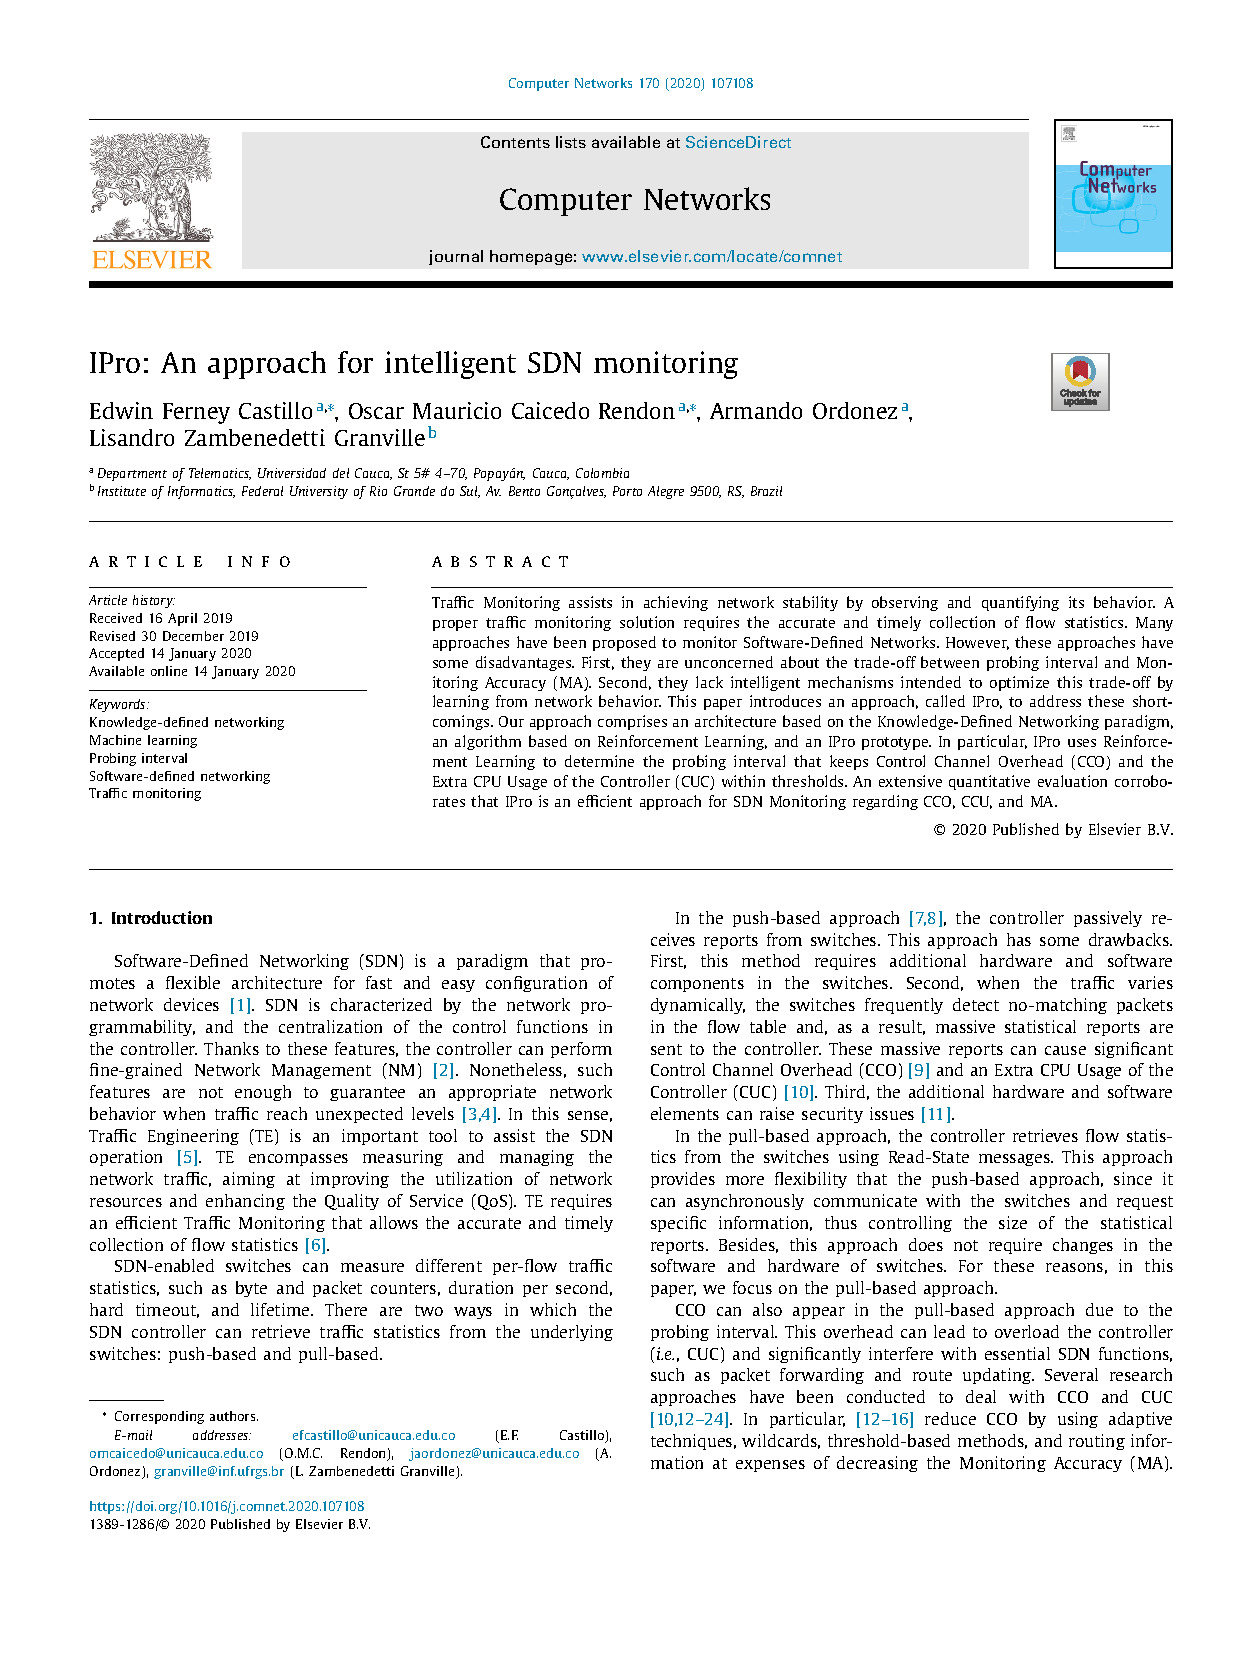
\includepdf[pages=-]{Anexos/IPro_Paper.pdf}
 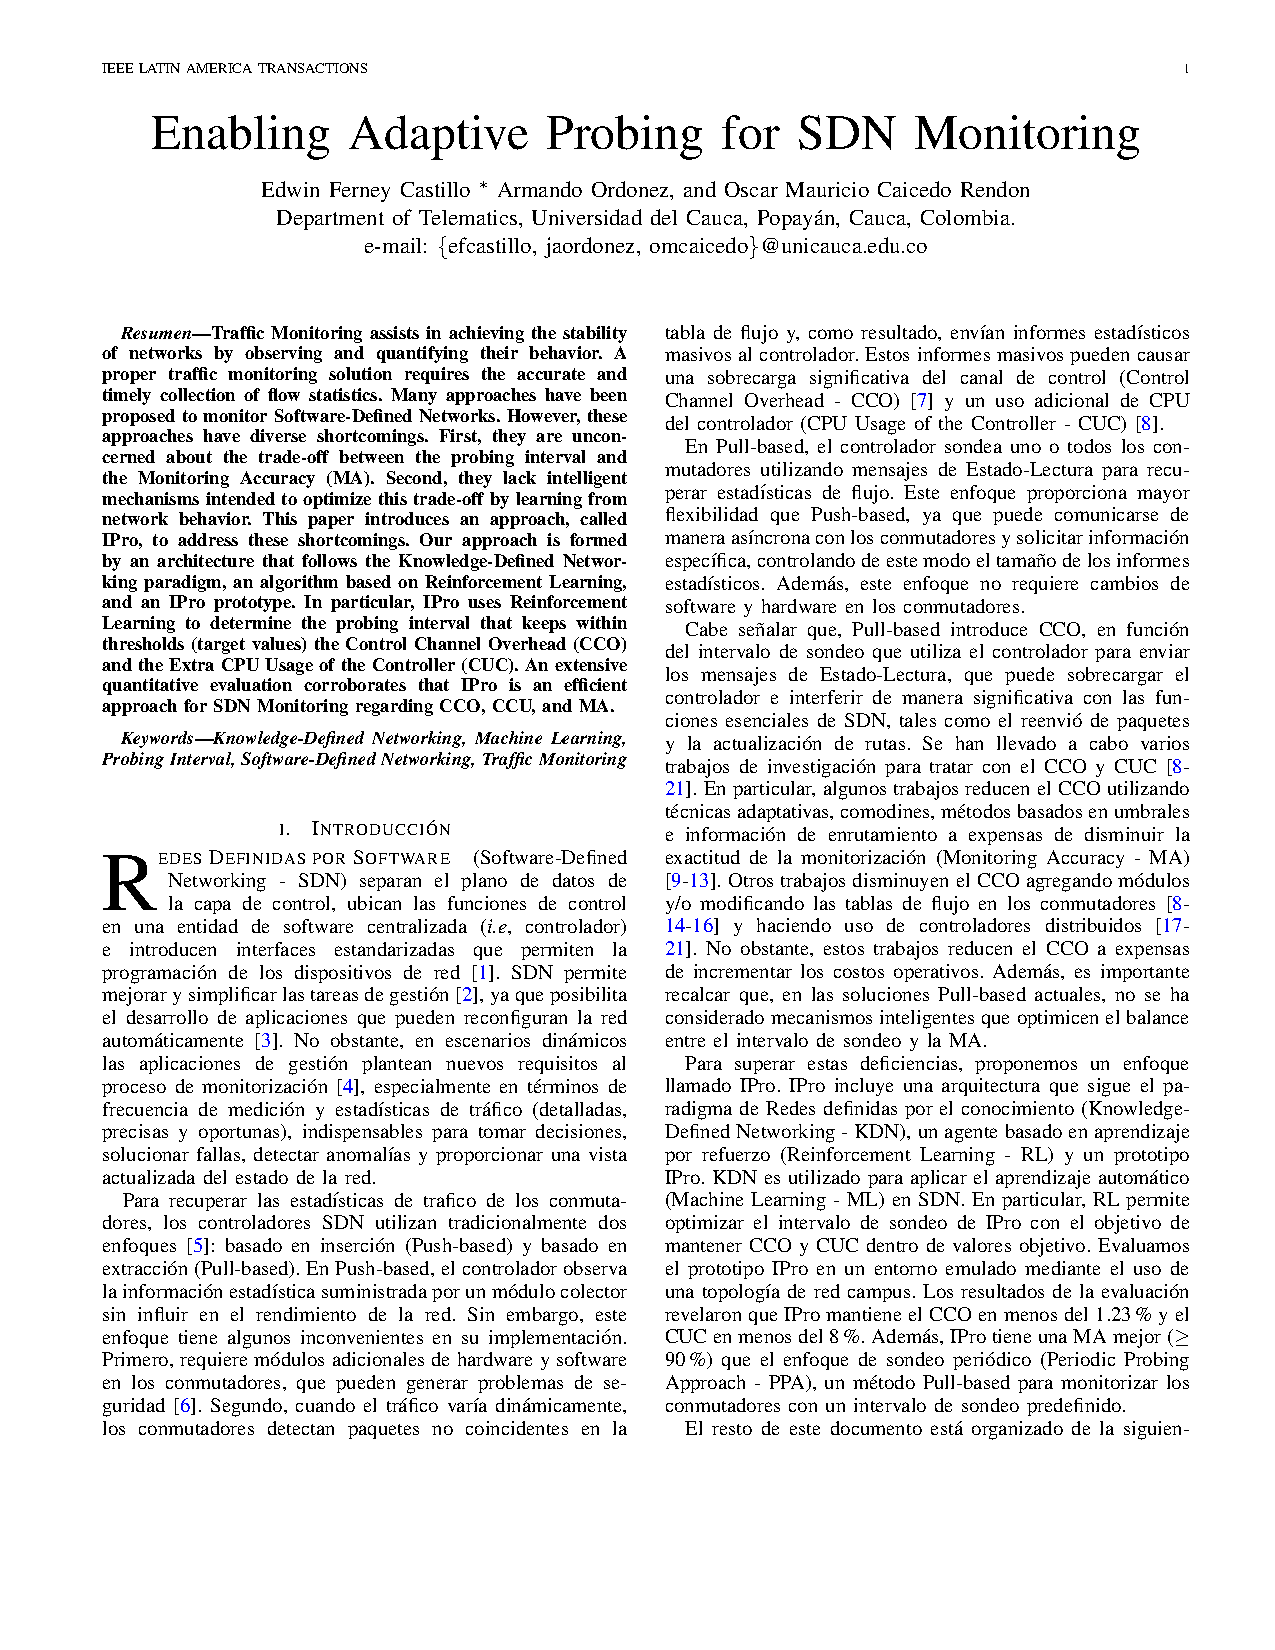
\includepdf[pages=-]{Anexos/IPro_LatinAmericaTransactions.pdf}